\section{Evaluation}
Zur Bewertung des vorgestellten Verfahrens wird besonderes Augenmerk auf schreibintensive Transaktionen, die Performance unterschiedlicher Transaktionstypen und Commit- und Abbruchraten gelegt.
Diese Eigenschaften werden wie zuvor beschrieben mit dem TPC-C Benchmark beobachtet.

\textbf{Schreibintensive Transaktionen:} Die im TPC-C Benchmark enthaltene Payment-Transaktion stellt eine besonders schreibintensive Anwendung dar, weshalb sie für diesen Test verwendet wird.
Dabei wurde zwar der gesamte TPC-C Mix ausgeführt, allerdings wurde nur die besagte Payment-Transaktion beobachtet.

\begin{figure}
	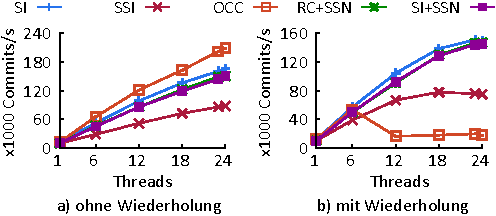
\includegraphics[width=\columnwidth]{img/Figure_3.pdf}
	\caption{Durchsatz der Payment-Transaktion des TPC-C Benchmarks}
	\label{fig:payment}
\end{figure}

Für eine differenzierte Betrachtung wurden zwei verschiedene Testszenarien beobachtet, wobei zum einen sämtliche Transaktionen, die abgebrochen werden mussten ohne eine Wiederholung fallen gelassen wurden.
Zum anderen wurde in einem Test die Performanz des Systems beobachtet wenn die fehlgeschlagenen Transaktionen direkt wiederholt werden bis diese abgeschlossen werden können.
Die Ergebnisse dieser Auswertung sind in Abbildung \ref{fig:payment} grafisch dargestellt.

Dabei fällt auf, dass die Verwendung von Read Committed in Verbindung mit dem Serial Safety Net einen Durchsatz leistet, der fast doppelt so groß ist wie der der Serializable Snapshot Isolation.
Der Grund dafür liegt laut den Autoren darin, dass der Hauptgrund für Transaktionsabbrüche bei der Verwendung von SSI in dem sogenannten Temporal Skew liegt.
Dabei versucht eine Transaktion eine Version zu überschreiben, welche nach ihrem Snapshot erstellt wurde, was bei SSI nicht zulässig ist.
RC hat damit kein Problem, da jederzeit auf die neueste Version zugegriffen wird, was sich auch durch die Erweiterung durch das SSN nicht ändert.

Außerdem ist zu erkennen, dass auch die Snapshot Isolation in Verbindung mit dem SSN eine hervorragende Performanz in beiden Testfällen besitzt.

Die Verwendung der Optimistic Concurrency Control zeigt bei dem Test ohne Wiederholungen die beste Performanz, da der gesamte Verwaltungsaufwand für die anderen CC-Verfahren entfällt.
Wird allerdings verlangt, dass die Transaktionen nach einem Abbruch wiederholt werden müssen, so sinkt der Durchsatz der OCC weit unter den Durchsatz der anderen CC-Verfahren, da die Zahl der zu wiederholenden Transaktionen so hoch ist, dass bei stark nebenläufigen Transaktionen die Performanz einbricht.